% ==============================================================================
% CAPÍTULO 3: EQUIPAMENTOS, SENSORES, ATUADORES E CONTROLADORES EM IRRIGAÇÃO IOT
% ==============================================================================

\begin{center}
\setstretch{1.0}
\textbf{\fontsize{14}{16}\selectfont CAPÍTULO 3}

\vspace{0.5em}

\textbf{\fontsize{14}{16}\selectfont EQUIPAMENTOS, SENSORES, ATUADORES E CONTROLADORES EM SISTEMAS DE IRRIGAÇÃO AUTOMATIZADOS}
\end{center}

\vspace{1.5em}

\section*{1. INTRODUÇÃO À HARDWARE E INSTRUMENTAÇÃO EM IRRIGAÇÃO IOT}

A automação do manejo de irrigação exige uma infraestrutura física composta por equipamentos eletrônicos, hidráulicos e mecânicos capazes de interagir diretamente com o ambiente agrícola. Enquanto os protocolos de rede e os softwares de backend gerenciam o fluxo lógico de informações, são os sensores, controladores e atuadores que traduzem instruções virtuais em ações físicas no campo.

Um sistema de irrigação inteligente opera em um ciclo contínuo de percepção, processamento e ação. Na etapa de percepção, os sensores medem variáveis físicas do solo e do microclima (como teor de umidade e temperatura). Na etapa de processamento, os controladores microprocessados analisam essas medições e decidem o momento exato e o volume de água a ser aplicado. Por fim, na etapa de ação, os atuadores elétricos e hidráulicos chaveiam motores e abrem válvulas para conduzir a água até as culturas.

Neste capítulo, são detalhados as principais plataformas de hardware embarcado, os sensores ambientais edáficos, os atuadores elétricos e hidráulicos, bem como os arranjos experimentais de laboratório utilizados no projeto e na construção de sistemas de irrigação automatizados com Internet das Coisas (IoT).

\newpage

\section*{2. CONTROLADORES E PLATAFORMAS EMBARCADAS (EDGE COMPUTING)}

O controlador embarcado é o cérebro eletrônico do nó de campo. Ele é responsável por executar o algoritmo de controle, ler os sinais dos sensores locais, acionar os relés e comunicar-se via rede sem fio com o servidor central HTTP.

\subsection*{2.1. Microcontrolador ESP32}

O microcontrolador ESP32 consolida-se como a principal plataforma de computação em névoa e borda (\textit{Edge Computing}) em projetos de Internet das Coisas agrícola. Equipado com um microprocessador Xtensa Dual-Core de 32 bits operando a frequências de até 240 MHz, o ESP32 integra nativamente conectividade Wi-Fi 802.11 b/g/n e Bluetooth v4.2 BR/EDR e BLE. A Figura 1 ilustra a estrutura física do módulo ESP32 utilizado no sistema de irrigação.

\vspace{1em}

\begin{figure}[h!]
\centering
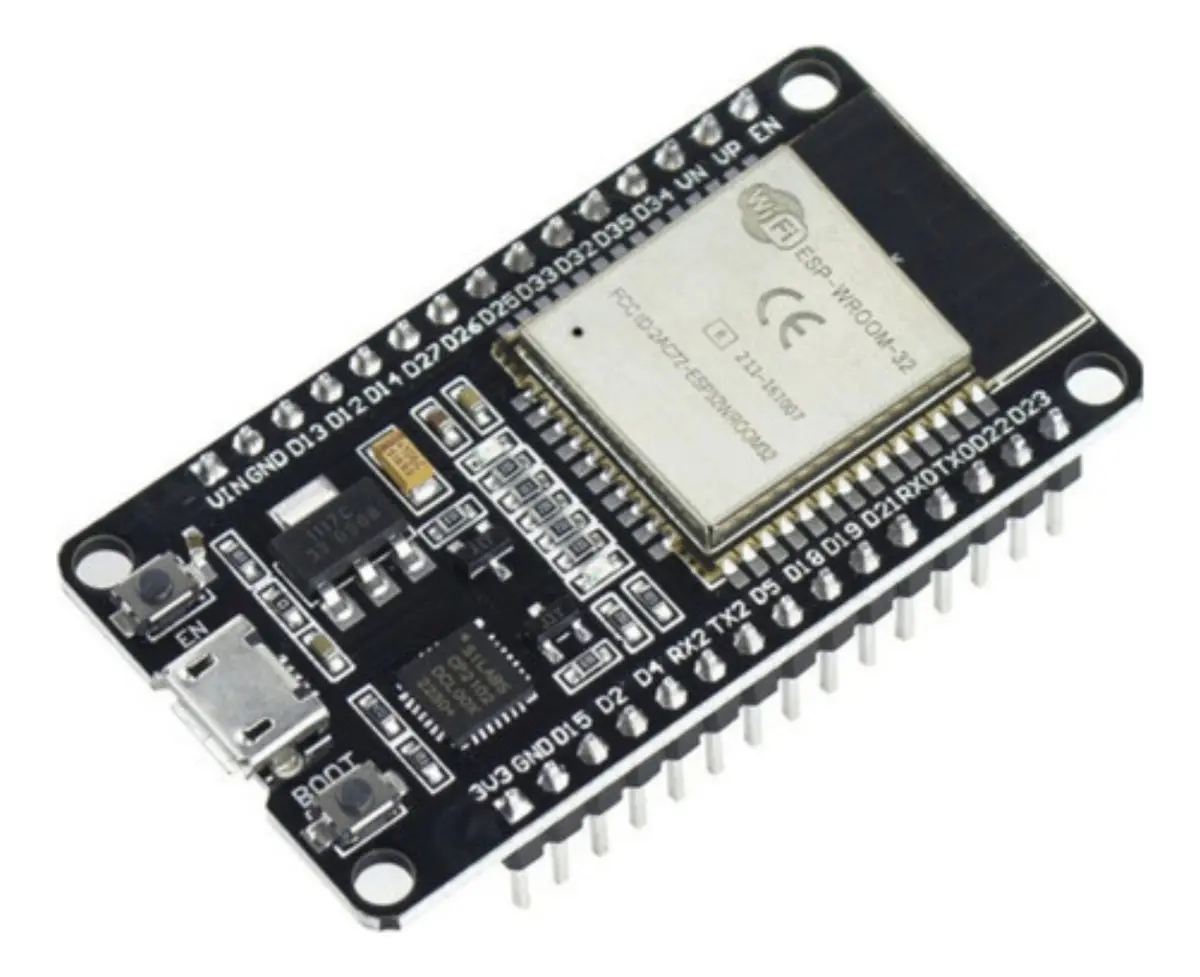
\includegraphics[width=0.45\textwidth]{images/esp32.png}
\caption{Módulo microcontrolador ESP32 com conectividade Wi-Fi e Bluetooth integrada para nós de controle de irrigação.}
\label{fig:esp32}
\end{figure}

\vspace{1em}

O ESP32 possui conversores analógico-digitais (ADC) de 12 bits para leitura de sensores edáficos, pinos com suporte a interrupções externas para medidores de vazão (pulsos de hidrômetros) e canais de modulação por largura de pulso (PWM) para controle de motores de velocidade variável. Sua capacidade de chavear modos de baixo consumo (\textit{Deep Sleep}), nos quais o consumo de corrente é reduzido a microamperes, viabiliza o uso do nó alimentado por pequenas baterias recarregáveis e painéis solares no campo.

\newpage

\section*{3. SENSORES AGRÍCOLAS DE CAMPO}

A coleta precisa de dados ambientais é indispensável para evitar tanto o estresse hídrico da cultura por subirrigação quanto o desperdício de recursos e a lixiviação de nutrientes por superirrigação.

\subsection*{3.1. Sensores de Umidade de Solo (Sensores Capacitivos)}

Os sensores de umidade do solo são transdutores desenvolvidos para estimar a lâmina de água contida nos poros da matriz edáfica. Diferente dos sensores resistivos convencionais, que sofrem corrosão acelerada por eletrólise e oxidação das hastes metálicas, os sensores de umidade do solo capacitivos operam pela variação da constante dielétrica do meio. A Figura 2 ilustra o sensor capacitivo de umidade do solo empregado nas parcelas agrícolas.

\vspace{1em}

\begin{figure}[h!]
\centering
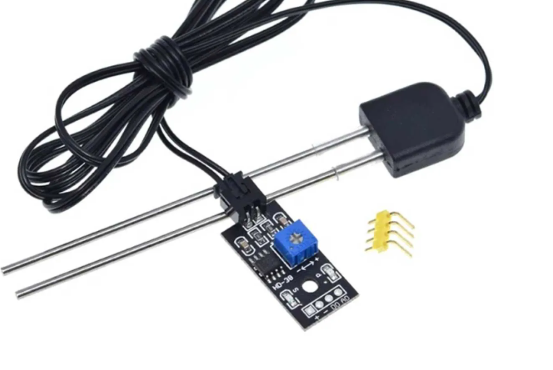
\includegraphics[width=0.38\textwidth]{images/sensor.png}
\caption{Sensor de umidade do solo capacitivo utilizado para amostragem edáfica em tempo real.}
\label{fig:sensor}
\end{figure}

\vspace{1em}

O circuito do sensor capacitivo gera um sinal de alta frequência e mede a alteração na capacitância provocada pela presença de água, já que a constante dielétrica do ar é aproximadamente 1, a do solo seco varia entre 3 e 5, e a da água pura é cerca de 80. O sinal analógico de saída é condicionado e lido pelos pinos ADC do microcontrolador ESP32, permitindo calibrar curvas de retenção de água específicas para o solo da fazenda.

\newpage

\section*{4. ATUADORES HIDRÁULICOS E DISPOSITIVOS DE CHAVEAMENTO ELÉTRICO}

Os atuadores são os elementos finais de controle que convertem os sinais de comandos emitidos pelos microcontroladores em trabalho físico, promovendo o deslocamento de fluídos e o acionamento de potências elétricas elevadas.

\subsection*{4.1. Válvulas Solenoides Hidráulicas}

A válvula solenoide é um atuador eletromecânico utilizado para interromper ou liberar a passagem de água nas tubulações dos setores de irrigação. Ela é composta por uma bobina elétrica (solenoide) e um corpo de válvula com diafragma interno. A Figura 3 ilustra uma válvula solenoide hidráulica para uso agrícola.

\vspace{1em}

\begin{figure}[h!]
\centering
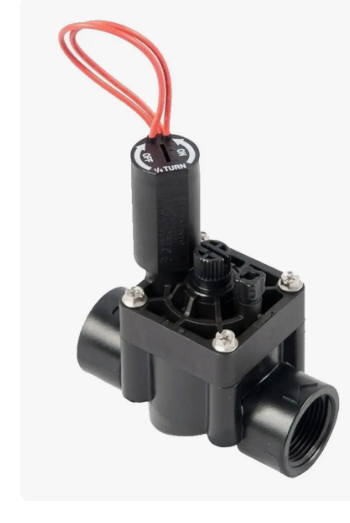
\includegraphics[width=0.38\textwidth]{images/solenoid.png}
\caption{Válvula solenoide de controle hidráulico para direcionamento do fluxo de água nos setores de plantio.}
\label{fig:solenoid}
\end{figure}

\vspace{1em}

Quando a bobina do solenoide é energizada pelo sinal elétrico do controlador, cria-se um campo magnético que atrai um êmbolo metálico interno, abrindo um pequeno orifício de alívio de pressão. Essa diferença de pressão sobre o diafragma faz com que a válvula se abra suavemente, evitando o golpe de aríete na rede hidráulica.

\subsection*{4.2. Bomba Hidráulica Principal}

A bomba hidráulica é o equipamento de pressurização responsável por captar a água do reservatório ou poço artesiano e recalcá-la até os emissores de irrigação (gotejadores ou aspersores). A Figura 4 apresenta a bomba hidráulica centrífuga acoplada ao sistema.

\vspace{1em}

\begin{figure}[h!]
\centering
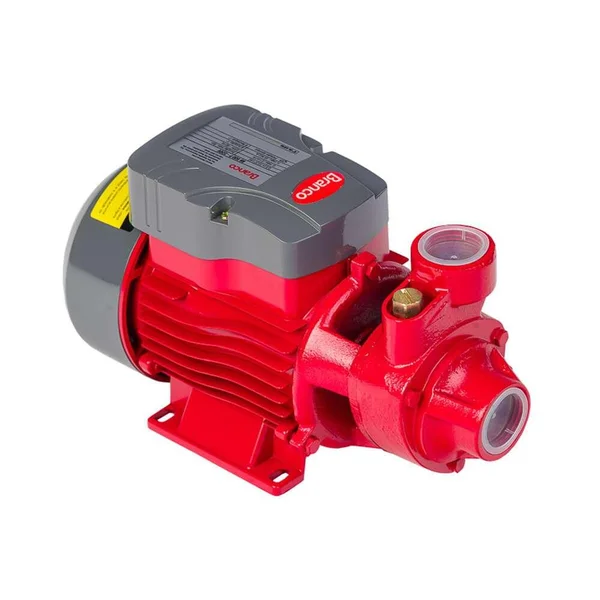
\includegraphics[width=0.38\textwidth]{images/bomba hidraulica.png}
\caption{Bomba hidráulica centrífuga para captação e pressurização da água no sistema de irrigação.}
\label{fig:bomba}
\end{figure}

\vspace{1em}

O dimensionamento da bomba hidráulica leva em consideração a vazão total exigida pelos setores em operação e a altura manométrica total do sistema, garantindo a pressão de serviço necessária para a uniformidade de distribuição de água no campo.

\subsection*{4.3. Módulos Relé e Chaves Contatoras Elétricas}

Devido à grande diferença de potência entre o microcontrolador ESP32 (que opera em 3.3V com corrente na casa dos miliamperes) e a bomba hidráulica (que exige tensão alternada de 110V/220V/380V e correntes elevadas), é indispensável utilizar elementos de isolamento e chaveamento elétrico intermediários.

O \textbf{Módulo Relé} de sinal, apresentado na Figura 5, utiliza um acoplador óptico para isolar galvanicamente o circuito sensível do microcontrolador da bobina do relé.

\vspace{1em}

\begin{figure}[h!]
\centering
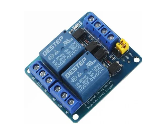
\includegraphics[width=0.35\textwidth]{images/rele.png}
\caption{Módulo relé optoacoplado para chaveamento de sinais elétricos de controle.}
\label{fig:rele}
\end{figure}

\vspace{1em}

Para motores de grande porte e motobombas trifásicas, o relé aciona a bobina de uma \textbf{Chave Contatora} industrial, ilustrada na Figura 6. A contatora possui contatos elétricos reforçados com liga de prata capazes de suportar surtos de corrente de partida de motores elétricos sem fundir ou gerar arcos elétricos danosos.

\vspace{1em}

\begin{figure}[h!]
\centering
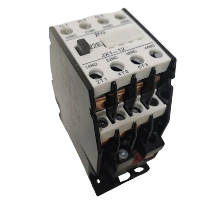
\includegraphics[width=0.35\textwidth]{images/contatora.png}
\caption{Chave contatora de potência industrial para acionamento seguro de motores e motobombas.}
\label{fig:contatora}
\end{figure}

\newpage

\section*{5. BANCADA EXPERIMENTAL DE LABORATÓRIO E AMBIENTE DE TESTES}

A validação do funcionamento integrado dos sensores, atuadores e controladores ocorre em bancadas de teste em ambiente de laboratório antes da implantação em campo definitivo. A Figura 7 mostra a bancada de prototipagem e testes de automação de irrigação.

\vspace{1em}

\begin{figure}[h!]
\centering
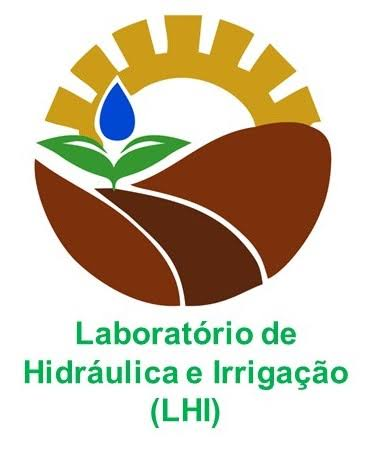
\includegraphics[width=0.45\textwidth]{images/laboratorio_irrigacao.png}
\caption{Bancada de testes de automação e instrumentação em laboratório de irrigação.}
\label{fig:lab}
\end{figure}

\vspace{1em}

O ambiente de testes permite simular diferentes cenários de umidade de solo, validar o tempo de resposta do chaveamento de solenoides, verificar a integridade da comunicação via HTTP/JSON e calibrar as salvaguardas de segurança.

Complementarmente, a Figura 8 detalha a montagem física dos componentes de controle em gabinete de proteção, enquanto a Figura 9 destaca o ambiente institucional de pesquisa e extensão tecnológica no qual a infraestrutura foi desenvolvida.

\vspace{1em}

\begin{figure}[h!]
\centering

\includegraphics[width=0.4\textwidth]{images/image.png}
\caption{Detalhamento da montagem física dos módulos de controle e atuadores em bancada.}
\label{fig:montagem}
\end{figure}

\vspace{1em}

\begin{figure}[h!]
\centering

\includegraphics[width=0.35\textwidth]{images/if_goiano.png}
\caption{Identificação da instituição de pesquisa e extensão tecnológica aplicadas ao agronegócio.}
\label{fig:inst}
\end{figure}

\newpage

\section*{6. SÍNTESE E ESPECIFICAÇÕES TÉCNICAS DOS EQUIPAMENTOS}

A Tabela 1 consolida as especificações operacionais dos principais equipamentos de hardware que compõem o sistema de irrigação inteligente.

\begin{table}[h!]
\centering
\fontsize{9}{11}\selectfont
\caption{Especificações técnicas e operacionais dos componentes de hardware do sistema de irrigação.}
\begin{tabular}{|p{3cm}|p{2.5cm}|p{3.5cm}|p{4cm}|}
\hline
\textbf{Equipamento} & \textbf{Categoria} & \textbf{Sinal / Tensão} & \textbf{Função Principal no Sistema} \\ \hline
ESP32 NodeMCU & Controlador & 3.3V DC / Wi-Fi 2.4 GHz & Executar o firmware de controle e gerenciar requisições HTTP REST. \\ \hline
Arduino UNO + W5100 & Controlador & 5V DC / Ethernet TCP & Efetuar leitura cabeada de sensores e transmitir pacotes via TCP bruto. \\ \hline
Sensor Capacitivo & Sensor & Analógico (0.5V -- 3.0V DC) & Mensurar a umidade relativa e a água disponível na matriz do solo. \\ \hline
Válvula Solenoide & Atuador & 24V AC ou 12V DC & Abrir/fechar o fluxo de água de setores individuais de irrigação. \\ \hline
Bomba Centrífuga & Atuador & 220V/380V AC Trifásico & Pressurizar a água do reservatório para os emissores de irrigação. \\ \hline
Módulo Relé 5V & Chaveamento & Sinal 5V DC / Contato 10A & Isolar o microcontrolador e acionar a bobina da contatora elétrica. \\ \hline
Chave Contatora & Chaveamento & Bobina 220V AC / 32A & Chavear com segurança a corrente elétrica de partida da bomba hidráulica. \\ \hline
\end{tabular}
\end{table}

\vspace{1.5em}

\section*{REFERÊNCIAS}

\begin{singlespace}
\noindent KRUGER, C. P. \textbf{Automação Agrícola e Internet das Coisas}: Aplicação de Sensores e Microcontroladores no Campo. São Paulo: Editora Técnica, 2024.

\vspace{0.8em}
\noindent SANTOS, T. R.; SILVA, M. A. \textbf{Sistemas de Irrigação Inteligentes baseados em ESP32 e Protocolos Web}. Revista Brasileira de Engenharia Agrícola e Ambiental, v. 28, n. 4, p. 210-225, 2025.

\vspace{0.8em}
\noindent TESTA, R.; GIANNOCCARO, G. \textbf{Precision Agriculture and IoT Sensors}: Engineering Principles for Automated Water Management. Agricultural Water Management, v. 260, p. 107-120, 2024.
\end{singlespace}
